% This example An LaTeX document showing how to use the l3proj class to
% write your report. Use pdflatex and bibtex to process the file, creating 
% a PDF file as output (there is no need to use dvips when using pdflatex).

% Modified 

\documentclass{l3proj}
\begin{document}
\title{Team V - How Not To Kill Your Dog}
\author{Ross Adam \\
        Andrew Gardner \\
        Nicole Kearns \\
        Mamas Nicolaou \\
        Asset Sarsengaliyev}
\date{18 March 2013}
\maketitle
\begin{abstract}

The abstract goes here

\end{abstract}
\educationalconsent
\tableofcontents

\chapter{Implementation}
\label{implementation}
\section{Abstract}
\section{Developing a Web Based Application }
One of the requirements for our project was that our final product should be available to 
use to any user with an Internet Connection. More specifically, any student should be 
able to access the application and practice on their drug calculations in their free time 
wherever they are with any device that can access the Web. This can be a laptop 
computer, a mobile phone or a tablet computer. \\ 
It was, therefore, clear to us that creating an application that needs to be installed on a 
machine in order to be usable was not an option. After a discussion with the team we 
decided that the most suitable solution would be to implement a application that would be 
accessible via a Web Browser. A web application would make it possible for any user to 
access our application from any device simply by navigating to our Web Applications 
URL address. \\ 

\subsection {Using a Web Application Framework}
After doing some research looking for the best possible option for developing web 
applications we decided that we would make use of a web development framework 
rather than writing the code for the whole application from scratch.
\subsubsection{ Developing from Scratch}
Developing an application from scratch has the potential to take up much needed time 
from the Development Phase. For each different page of an application there needs to be 
a unique file (for example an html document) that will be sent to the client's web browser 
when the page is called. An application usually has the same layout on every page with 
basic components, like the applications logo or the applications default buttons, being 
displayed on each page. It is therefore clear that having a separate file to correspond to 
each different page of an application can lead to a lot of coding overhead and 'boiler 
plate' code. In the case of a change request, a developer will need to modify the code in 
each different page separately which would take much of our development time. Time was a major concern for us as we only had a limited amount of time to get the application designed, developed, evaluated and delivered to our client.
\subsubsection{Developing with a web application framework}
A Web Application Framework is a set of prefabricated software building blocks that 
programmers can use, extend, or customise for specific computing solutions" (Leif 
Azzoperdi, DIM3 Lecture 3). A framework would allow us to start implementing our 
application with a concrete base to support us by providing default functionality whilst 
allowing us to extend or override functionality to suit our specific requirements. "One 
significant advantage to using a framework is that you're required to write only a 
minimal amount of code to get up and running from scratch"(Professional Python 
Frameworks: Web 2.0 Programming with Django and Turbogears page 48). This was 
one of the most important reasons for which we opted in using a Web Application 
Framework for our project. Afterwards, there was one more decision that needed to be 
undertaken. There are a number of frameworks available on the web so we had to decide 
on one of them before starting our implementation. 
\subsection {Which framework to use?}
We came down to three popular web application frameworks that would help us develop 
our software but we had to decide on one of them. Our supervisor suggested that three 
of us take one of the three frameworks each and try to build a simple application in one 
week. This would not only show us what can be built with that particular framework but 
it would also show us how long it take for a developer to learn how to use the 
framework, and how much can be built in a week by using that framework. The three 
options were 
\begin{itemize}
\item Web2Py 
\item Django 
\item Ruby on Rails 
\end{itemize}
After our frameworks evaluation we came to the following conclusions about them: 
Ruby on Rails offers useful code generators which can produce functions out of one line 
of code written by the developer and has a build in testing framework which can be 
particularly useful for our testing. However, the mystery behind the code generators can 
cause confusion to developers and thus increase development time. \\
Web2Py uses a Python-based template language and supports development from a Web 
Browser. We have been using python for our introduction to programming course in Level 
1 of our university studies so it would python is a language we have all used and are 
comfortable with. Moreover, a developer needs not have their own computer with them 
to work on the development of the application. Web2Py gives the ability to a developer 
to work on the code of the application via a web interface which can be particularly 
useful in case one of the team members is traveling and is not able to use their own 
computer to work on application. \\
Django is an MVT (Model, View, Template) based framework that runs with Python on 
its back end. This gives us the advantage of having separation of concerns in our 
application since different components in the framework act independently from each 
other so a developer can work on one part of the application while another can work on 
a different component without having to wait for a different component to be completed. 
Django is an extremely customisable framework since it comes packed with a lot of 
functionality which can be used out of the box or can be further modified to reflect our 
goals and objectives. On the other hand it might take time to learn since it has its own 
way of doing things and a developer needs to adapt to it.

\subsection {Why Django}
We decided to use Django since it gives us great flexibility as to what our end product 
can be like, it is documented extremely well online and even though learning it can take 
some time, we consider it to be a well worth investment since we will have to use 
Django in one of our courses in second semester as well. 
\section{Development in Django}
As its being described on djangoproject.org, Django is "The Web framework for 
perfectionists with deadlines". It is a rapid web development framework that can save 
you the trouble of writing repetitive boilerplate code. A developer using Django can 
achieve greatness with minimal coding. Django comes with an object relational mapper 
which means that we can define our database schema in Python code by defining 
classes and Django will then produce an sql code that can be injected in our database 
with minimal effort from the developer in order to create any tables required for the 
project. It has a dynamic build in administration interface which can be customised 
according to our needs. This can be used, in our case, as a way for a Course 
Coordinator or a Tutor to create new topics, add slides and questions to each topic, 
create questions for the final assessment page and create new users or groups of users 
with special permissions. This will be discussed further in this report.
\subsection{The MTV Model}
The MTV model used by django is a development mode very similar to the MVC model which is widely used by a number of web application 
frameworks such as Backbone.js SproutCore and the Cocoa framework used in Mac OS X and iOS applications. Django, since it likes to do things its own way, uses a "modified" version of the MVC model. Its model is called MTV (Model, Template, View). The model in the MVC 
plays the same role as the model in MTV which is sensible. However, the "View" in the 
MTV maps to the "Controller" of the MVC and the "Template" of the MTV maps to the 
MVC's "View". Of course this is slightly complicated so it might cause some confusion to 
a developer coming from an MVC background. 
The MTV in general defines the way everything works in Django. Everything in Django 
can be broken down to 3 components; The Models, the Templates and the Views.
\subsection{Models}
"A model is the single, definitive source of data about your data. It contains the essential 
fields and behaviours of the data you are storing"(Django website). In other words, any a 
table in the database can be created by defining a model in the Models.py file. A 
database field for that table can be defined as an attribute of the corresponding model. 
The command "manage.py syncdb" will then read the Models.py file create an SQL code 
and then run it agains the applications database to create any tables defined by the 
developer. 
For example if the code in picture below is run it will create a Database table of topics 
where each topic has a title and a publication date. \\
class Topic(models.Model): \\
title = models.CharField(max\_length=100) \\
pub\_date = models.DateTimeField('Date Published')\\
\subsection{Views}
A view takes care of what is sent to a browser when a specific URL is requested. It is 
responsible for making any requested action as this is defined in the tags of the html 
page associated with each view. Such actions might be read or write to the database 
commands or any other actions that are required by a page.
\subsection{Templates}
A template is usually an html file. It is the base of what will be send on to a web browser 
client. It described how the data should be presented to the user and can contain a 
number of Django tags and variables. A tag is surrounded by "" and tells 
Django that a special action needs to be taken at that point of the page. This special 
action can be an "if" statement, a "for" loop etc. A variable is simply telling Django to load 
a specific value from the Database and display it at this point of the page. Templates are 
used by Django as the model for a page to be sent to a web client.
\subsection{Controller}
Each Django application has a "urls.py" file which holds definitions that will be matched 
against requests by web clients. An example url definition in "urls.py" could be \\
\verb|"url(r ^'contents', 'views.contents')"|. \\In this scenario if our server is hosted on 127.0.0.1 
port 8000 and a client requests "127.0.0.1:8000/contents" Django will match the 
request with the definition in "urls.py" and call the appropriate view which is the second 
argument of the url() function. In this case it will be the "contents" view.
\section{3-Tier Architecture}
For our implementation we used a 3-Tier Architecture.
\subsection{N-Tier Architecture Diagram}
 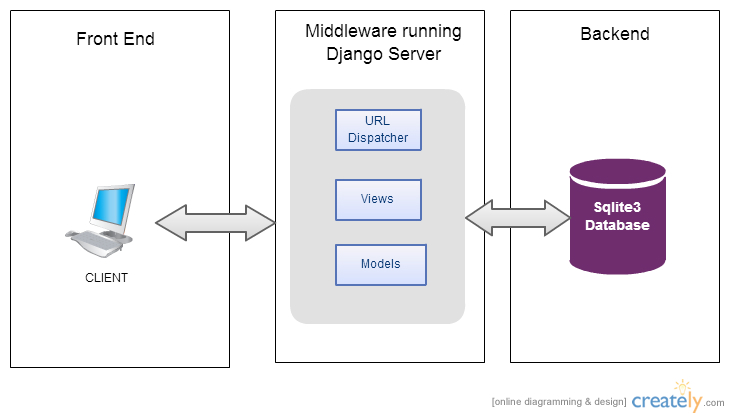
\includegraphics[width=\linewidth]{images/ntier.jpg}
\subsection{Front End}
The application can be accessed by any user with a web browser such as Internet 
Explorer, Google Chrome, Mozzila Firefox, Safari and so on. \\
\subsection{Middleware}
This is our Django server. Responsible for matching requests from Clients using the 
URL dispatcher which in return calls the appropriate View which then fetches any 
required context from the Models.py and our Backend Services. 
\subsection{Back End}
This is our Sqlite3 Database. Other database options included MySQL, Oracle or 
PostgreSQL. However we opted in for Sqlite3 since it offers all the functionality we 
need and Django provides more support for it as it is its default option. \\
\section{Back End}
\subsection{Topic}
\begin{tabular}{|c|c|c|}
\hline \textbf{Field Name} & \textbf{Type} & \textbf{Notes}\\
\hline title & CharField & 1000 characters max \\ 
\hline pub\_date & DateTime &  \\ \hline
\end{tabular}
\subsection{Question}
\begin{tabular}{|c|c|c|}
\hline \textbf{Field Name} & \textbf{Type} & \textbf{Notes}\\
\hline qTopic & ForeignKey & Points to a Topic object \\ 
\hline text & CharField & 1500 characters max \\
\hline answer & CharField & 100 characters max \\ \hline
\end{tabular}

\subsection{FinalTestQuestion}
\begin{tabular}{|c|c|c|}
\hline \textbf{Field Name} & \textbf{Type} & \textbf{Notes}\\
\hline text & CharField & 2000 Characters max length \\ 
\hline answer & CharField & 100 characters max \\ \hline
\end{tabular}

\subsection{Slide}
\begin{tabular}{|c|c|c|}
\hline \textbf{Field Name} & \textbf{Type} & \textbf{Notes}\\
\hline sTopic & ForeignKey & Points to a Topic object \\ 
\hline image & ImageField &  \\ \hline
\end{tabular}

\section{Managing the Front End}
The way Django is generally managing the Front End of an application is quite 
straight forward. It simply takes a predefined template (html file), adds any required 
content from the models (database objects) and sends the file over to a web browser. 
However creating simple html files and feeding them the data from our models is not 
enough to produce a high quality web application. The fact that we were not 
experienced in web application was not helping us find a solution without investing 
some time on researching. In our quest to find a way to manage the front end design 
we looked at a number of solutions. Some of them were the "Backbone.js", "Tastypie" 
and "Pyjamas". At a first glance each of these frameworks seemed promising. 
However, trying to use them to produce high quality front end design became more of 
a time wasting challenge rather that a time worthy investment.
\subsection{Possible frameworks for Front End management}
\subsubsection{Backbone}
As its website states, "Backbone.js gives structure to web applications by providing 
models with key-value binding and custom events, collections with a rich API of 
enumerable functions, views with declarative event handling, and connects it all to 
your existing API over a RESTful JSON interface". Fair enough, now how can we 
proceed and use this Framework with our Django application? A number of github 
repositories were available online, all with example applications using Backbone. 
However, since all of them were out of date and description for Backbone and 
Django integration was vague at best, we soon abandoned the idea of using 
Backbone. 
\subsubsection{Tastypie}
TODO!
\subsubsection{Pyjamas}
Pyjamas is a framework which takes code written in Python and translates that 
into javascript and jquery code without the need of having a developer experienced 
in using javascript and jquery. We managed to get Pyjamas set up successfullly, 
but the result was not exactly what we expected. The design looked poor and we 
had to invest even more time in advancing our skills on coding a GUI with python
\subsubsection{Compination of traditional Django friendly frameworks}
TODO! 
\section{Middleware: Linking the back with the front}
Talk about how the Django server makes the connection between the front end and the back end.
\section{Message Passing}
\subsection{Database Request Format}
Database requests description and sequence diagram
\subsection{Answer Validation Request}
Answer validation request description and sequence diagram
\subsection{Topic Related Data Request}
Topic Related Data request and sequence diagram
\section{End Product}
\subsection{Desired Functionality}
How the desired functionality mentioned in Requirements and Design sections was realised through the implementation
\subsubsection{Welcome Page}
How the Welcome page is implemented
\subsubsection{Topic Page}
How the topic page is implemented
\subsubsection{Contents Page}
How the content page is implemented
\subsubsection{Final Assessment Page}
How the final assessment page is implemented
\subsubsection{Administration Page}
How the administration page is implemented
\subsection{Interaction Diagrams}
\subsubsection{Topic Page}
Interaction diagram for communications and message passing between the Topic page and the server.
\subsubsection{Contents Page}
Interaction diagram for communications and message passing between the Contents Page and the server
\subsubsection{Final Assessment Page}
Interaction diagram for communications and message passing between the Final Assessment Page and the server
\section{Challenges and Solutions}
Talk about the risks and challenges faced during the development phase of the project and how these were faced.
\section{Known Issues}



\end{document}
